\documentclass[11pt, a4paper, final]{article}
\usepackage{tmh}
\usepackage{bbm}
\renewcommand{\labelenumi}{\roman{enumi})}
\renewcommand{\phi}{\varphi}

\renewcommand{\P}{\mathbb{P}}
\newcommand{\E}{\mathbb{E}}
\renewcommand{\R}{\mathbb{R}}
\newcommand{\T}{\mathbb{T}}
\newcommand{\Z}{\mathbb{Z}}
\newcommand{\F}{\mathcal{F}}
\newcommand{\Dt}{\Delta t}
\newcommand{\Dv}{\Delta v}
\newcommand{\Dx}{\Delta x}
\newcommand{\dx}{\dif x}
\newcommand{\dt}{\dif t}
\renewcommand{\familydefault}{\sfdefault}
\usepackage[scaled]{helvet}
\setlength{\parindent}{0em}
\setlength{\parskip}{1em}

\usepackage{showkeys}

\title{{\huge Interacting Particle Systems} \\\vspace{1cm} Subtitle}
\author{Thomas M. Hodgson\\ \vspace{0.5cm} Maxwell Institute}
\date{\today}

\begin{document}

	\maketitle
    \thispagestyle{empty}
	\newpage
	\tableofcontents
	\listoffigures
	\newpage
    
	\section{Introduction}\label{sec:introduction}
        +++Motivation, particle systems and flocking in biology+++
       
	\section{The Model}\label{sec:model}
        		We here introduce the model of Butt\`a, Flandoli, Ottobre and Zegarlinski \cite{Butta2019}. This is a Vicsek-type continuum model for an interacting particle system. There are three key parts to this model that together create interaction and ordered motion: a herding function, denoted $G$; an averaging function, denoted $M$; and an interaction function, $\phi$. Each will be described before the full model is introduced. Throughout, we will be considering the phase space distribution function $f_t(x,v)$, where $(x,v) \in \T \times \R$ and $t \in \R$ with $\T \cong \R \backslash \Z \cong S^1$ denoting the unit one-dimensional torus. The distribution function represents the density of particles at time $t$ at a given point in phase space $(x,v)$.
		
		The interaction function, $\phi: \T \to \R $ acts on the smallest scale, between individual points. It is smooth and satisfies the following:
		\begin{align}\label{eq:phi}
			\phi(x) \geq \epsilon >0, && \phi(x) = \phi(-x), &&& \int_{\T} \phi(x) \dif x = 1.
		\end{align}
		These are quite natural ways to describe an interaction. The first means that all points interact with each other to some degree. The second requires symmetry when interacting, and finally the function must have unit integral -- this is only for simplicity and could in fact be any value, so long as it is finite. For example, we may take $\phi \equiv 1$. This will satisfy the above requirements and corresponds to all points interacting an equal amount, regardless of position on the torus. This will create space-homogeneity, which we will return to later.
		
		The function $M:\R \to \R$ takes a weighted average of the interactions across the space.	
		\[ 
			M(t,x) = \frac{\int_{\T}\int_{\R}f_t(y,w)\phi(x-y)w\dif w \dif y}{\int_{\T}\int_{\R}f_t(y,w)\phi(x-y)\dif w \dif y}
		\]
		The interaction function provides the weighting. Note the argument of  $\phi$ is the distance between two points in space and also that $M$ depends on $f_t$. The denominator is required in the corresponding particle model to prevent the size of the group of particles from having an effect on the dynamics. It can be thought of as a normaliser.
		
		Finally, the herding function $G:\R \to \R$ is chosen such that
		\begin{align*}
			&G(u)=-G(-u),&& {\begin{cases}
								G(u)>u & \text{ if } 0< u <1\\
								G(u)<u & \text{ if } u > 1
				   		   \end{cases}}.
		\end{align*}
		We shall consider three forms of $G$.
		\begin{enumerate}
			\item Step:
			\[
				G(u) = \frac{1+\beta \mathrm{sgn}(u)}{1+\beta}, \qquad \beta > 0	
			\]
			This is the usual choice in the biological literature, with \(\beta = \frac{1}{2}\). It is differentiable everywhere with $G'(u) = \frac{1}{1+\beta}$, except at $u=0$. This discontinuity makes analysis more difficult.
			\item Smooth:
			\[
				G(u) = \frac{\arctan(u)}{\arctan(1)}
			\]
			Here we get a much smoother curve that is everywhere differentiable. However the gradient isn't very steep and there is no way to control the shape of the curve.
			\item Sigmoid:
			\[
				G(u) = \frac{2}{1+\mathrm{e}^{-\alpha u}} - 1 , \qquad \alpha >0
			\]
			The sigmoid herding function provides a middle ground between the previous two. It is smooth, but can be made as sharp as required by adjusting the parameter $\alpha$. However note that it only satisfies second requirement above in the limit as $\alpha \to \infty$ as the function is bounded above by 1.
		\end{enumerate}
		During the analysis, we will use the smooth herding function for its amenability. The role of $G$ is to herd the mean velocity towards a fixed value -- in this case plus or minus one. How it does so will become clearer when we discuss the dynamics of the model.
        \begin{figure}
            \centering
            \includegraphics[width=\linewidth]{Figures/herdingfunctions}
            \caption{Step, smooth and sigmoid herding functions, with the dashed line $y=x$ for reference}
            \label{fig:herdingfunctions}
        \end{figure}
		We now have all the necessary ingredients to give the full continuum model. The evolution of the distribution is described by
		\begin{equation}\label{eq:fullPDE}
			\partial_t f_t(x,v) = -v\partial_x f_t(x,v)  +\partial_v v f_t(x,v) - \partial_v \left[ G(M(t,x))f_t(x,v)\right] + \sigma \partial_{vv}f_t(x,v),
		\end{equation}
		where $\sigma > 0$ is a constant describing the rate of diffusion. At its heart, this is just an advection-diffusion equation. The first term illustrates the movement around the torus, the second describes a damping effect and the fourth gives a diffusive effect in velocity. The third term is where the interest lies as it contains all the information on interaction and herding.
		
        
	\section{Dynamics}\label{sec:dynamics}
        		To better understand the dynamics of \eqref{eq:fullPDE}, first let $G\equiv0$. This removes any interaction between particles and the equation becomes
		\begin{equation}\label{eq:OU_FPE}
			\partial_t f_t(x,v) = -v\partial_x f_t(x,v) +\partial_v vf_t(x,v) + \sigma \partial_{vv}f_t(x,v).
		\end{equation}
		This is the Fokker-Planck equation for the following system:
		\begin{equation}\label{eq:2d_OU}\begin{cases}
			\dif x_t = v_t\dif t\\
			\dif v_t = -v_t\dif t + \sqrt{2\sigma} \dif W_t. 
		\end{cases}	\end{equation}
		Here, $W_t$ is a standard one-dimensional Wiener process. We recognise this as overdamped Langevin dynamics, and so we can exactly calculate the unique invariant measure. To do so it is necessary to solve $\partial_t \rho_t = 0$, that is, when is the density not changing in time. The evolution in $v$ is described by an Ornstein-Uhlenbeck process so it is known that the unique stationary distribution is Gaussian with mean $1$ and variance $\sigma$. The position $x$ depends only on $v$ with no noise. There is no reason to assume any sort of mean reverting behaviour and expect the density to spread out uniformly on the torus. A guess at the solution would then be $\rho (x,v) = \frac{1}{2\pi}\exp(\frac{-v^2}{2})$, with some normalising constant. Notice that this equation does not depend on $x$. By substitution into the stationary Fokker-Planck equation, this is indeed a solution.
        
        Similarly, when $G\not\equiv 0$ the density $f_t(x,v)$ of \eqref{eq:fullPDE} is the Fokker-Planck equation of the two dimensional SDE,
		    \begin{equation}\label{eq:McK_V}\begin{cases}
		    \dif x_t = v_t\dif t\\
		    \dif v_t = \left[G(M(t,x_t))-v_t\right] \dif t + \sqrt{2\sigma} \dif W_t. 
			\end{cases} \qquad  (x_t,v_t) \in \T \times \R
			\end{equation}
		This is a McKean-Vlasov equation as the function $M(t,x_t)$ conceals a dependence on the law of the process. 
        \[
            M(t,x) = \frac{\E\left[ v'_t \phi(x-x'_t)\right]}{\E\left[\phi(x-x'_t)\right]}
        \]
        The pair $(x'_t,v'_t)$ is a random variable equal in distribution to $(x_t,v_t)$. This representation of $M(t,x)$ is the same as the one given previously, however in this setting it is natural to use expectation notation over integrals. To illustrate the necessity of introducing another random variable, albeit one that is equal in law, consider the case when the interaction function is the indicator on the interval $[-b,b]$, $\phi(x) = \mathbbm{1}_{[-b,b]}(x)$. This does not meet the requirements in Section \ref{sec:model}, in particular it is neither strictly positive nor does it have unit integral. 
        \begin{align*}
            M(t,x) &=  \frac{\int_{\T}\int_{\R}f_t(y,w)\phi(x-y)w\dif w \dif y}{\int_{\T}\int_{\R}f_t(y,w)\phi(x-y)\dif w \dif y}\\
            &=  \frac{\int_{\T}\int_{\R}f_t(y,w) \mathbbm{1}_{[-b,b]}w\dif w \dif y}{\int_{\T}\int_{\R}f_t(y,w) \mathbbm{1}_{[-b,b]}\dif w \dif y}\\
            &= \frac{\E\left[ v'_t \mathbbm{1}_{[-b,b]}\right]}{\P(x' \in \left[x-b,x+b\right])}\\
            &= \E\left[ v'_t|x' \in [x-b,x+b] \right]
        \end{align*}
        It makes no sense to consider $\P(x \in [x-b,x+b])$ as it is always equal to one so the auxiliary variable $(x'_t,v'_t)$ is used. +++More detail?+++ This calculation also illustrates how $\phi$ describes the interaction or `where to look' while $M$ acts as a average velocity of the points `within range'. The transport term, $\partial_v\left( \left[ v-G(M(t,x))\right]f_t(x,v)\right)$ then acts to change the velocity towards the local average given by $M$. It is in this sense that $G$ is the herding function `herding' the system towards a common velocity.
        
        The McKean-Vlasov representation of the system is also the weak limit of an $N$-body particle system described by
        \begin{equation}\label{eq:full_particle}\begin{cases}
            \dif x^{i,N}_t = v^{i,N}_t\dif t\\
            \dif v^{i,N}_t = -v^{i,N}_t\dif t + G\left(\frac{\frac{1}{N}\sum_{j=1}^N \phi(x_t^{i,N} - x_t^{j,N})v^{j,N}_t  }{\frac{1}{N}\sum_{j=1}^N \phi(x_t^{i,N} - x_t^{j,N})}\right)\dif t + \sqrt{2\sigma} \dif W^i_t 
            \end{cases}, \qquad  i = 1,\dots,N.
        \end{equation}
        This gives another view of the full system \eqref{eq:fullPDE}, and one that is particularly amenable to analysis. It also allows a more intuitive view of the system -- rather than thinking of how a density changes over time, we can think of particles moving around a torus and interacting according to $\phi$.
        
        \subsection{Invariant Measures under Space Homogeneity}
        Thus far, we have found the invariant measure for only the rather uninteresting case when $G \equiv 0$. To progress further, we must simplify the system. One way to do this is to impose that the density does not depend on the position in space and set $\phi \equiv 1$. The weighted local average velocity $M$ becomes neither local nor weighted. In the particle system, this means that each particle interacts with every other particle, irrespective of the distance between them. Indeed,
        \begin{align*}
            M(t,x) =&  \frac{\int_{\T}\int_{\R}f_t(y,w)\phi(x-y)w\dif w \dif y}{\int_{\T}\int_{\R}f_t(y,w)\phi(x-y)\dif w \dif y}\\
            =&  \frac{\int_{\T}\int_{\R}f_t(y,w)w\dif w \dif y}{\int_{\T}\int_{\R}f_t(y,w)\dif w \dif y}\\
            =& \int_{\T}\int_{\R}f_t(y,w)w\dif w \dif y\\
            :=& \langle w \rangle_{f_t}.
        \end{align*}
        So the weighted local average velocity is just the average of the distribution $f_t(v)$ or equivalently, the average velocity of all particles in the system. The evolution is then described by
        \begin{equation}\label{eq:space_hom_PDE}
            \partial_t f_t(v) = \partial_v vf_t(v) - \partial_v G(\langle w \rangle_{f_t})f_t(v) + \sigma \partial_{vv} f_t(v).
        \end{equation}
        The above problem's well-posedness can be shown as follows. Let
        \[
            h_t(v) = f_t(u),\text{ where } u = v + \int_0^t G(\langle w\rangle_{f_t}) \dif s.
        \]
        To find an equation that $h_t(v)$ solves, we use the chain rule.
        \begin{align*}
            \partial_t f_t(u) &= \partial_t f_t(u) +  G(\langle w\rangle_{f_t})\partial_v f_t(u) && \text{as   } \pd{g}{v} = 1, \pd{g}{t} = G((\langle w\rangle_{f_t})\\
            &=\partial_v vf_t(u) - \partial_v G(\langle w \rangle_{f_t})f_t(u) + \sigma \partial_{vv} f_t(u) + G(\langle w\rangle_{f_t})\partial_v f_t(u) &&\text{as  } f_t \text{ solves } \eqref{eq:space_hom_PDE}\\
            &=\partial_v vh_t(v) + \sigma \partial_{vv} h_t(v) , \qquad h_0(v) =f_0(v).
        \end{align*}
        So $h_t$ solves the Fokker-Planck equation for the one-dimensional Ornstein-Uhlenbeck process which is well posed +++cite+++. Therefore the solution $f_t(v)$ of \eqref{eq:space_hom_PDE} exists and is unique given initial data. To find invariant measures of this evolution, set the transient term to zero and solve the remaining PDE, which can be written in gradient form. First note that if $G\equiv 0$, this system for $f_t$ is the same as that for $h_t$, and so has a unique invariant measure $\mathcal{N}(0,\sigma)$. When the herding function is non-zero, other measures are also stationary as we will now show. For brevity, we omit the dependence on $v$ of $f$ and write $\langle w \rangle_{f_t} = M_1$. The latter is natural as it denotes the first moment of the distribution.
        \begin{align*}
            &\partial_v\left[(-G(M_1) +v) f + \sigma \partial_v f \right] = 0\\
            \implies& (-G(M_1) +v) f + \sigma \partial_v f = C_1
        \end{align*}
        This ODE is solvable and gives 
        \[
            f(v) = C_2\exp\left(\frac{2G(M_1)v - v^2}{2\sigma} \right). 
        \]
        Applying the constraint $\int_\R f(w)\dif w = 1$ gives $C_2 = \exp(-G^2(M_1))/\sqrt{2\pi\sigma}$. +++note here this is a Gaussian with mean $G(M_1)$? Immediately implies that $M_1 = G(M_1)$ without need for integration +++ Furthermore, from the definition of space average,
        \begin{align*}
            M_1 :=& \int_\R wf(w) \dif w\\ 
            =& \int_\R \frac{w\exp(-G^2(M_1))}{\sqrt{2\pi\sigma}} \exp\left(\frac{2G(M_1)v - v^2}{2\sigma} \right)\\ 
            =& \int_\R \frac{w}{\sqrt{2\pi\sigma}} \exp\left(\frac{ - (v-G(M_1))^2}{2\sigma} \right)\\
            =& G(M_1)
        \end{align*}
        Using the smoothed version of the herding function from Section \ref{sec:model} gives $G(M_1) = 0, \pm 1$. Substituting this into our expression for $f$ gives three invariant measures:
        \begin{align*}
            \rho_0 &= \frac{1}{\sqrt{2\pi\sigma}}\exp\left(-\frac{v^2}{2\sigma} \right), && \rho_{\pm} = \frac{1}{\sqrt{2\pi\sigma}}\exp\left(-\frac{(v\pm 1)^2}{2\sigma}\right).
        \end{align*}
        These are Gaussian densities with mean $0, \pm 1$ and variance $\sigma$.
        
        We have found three invariant measures for the evolution \eqref{eq:space_hom_PDE}, however whether the system will converge to these distributions given initial data remains to be settled. In the space homogeneous case it is possible to close equations on the moments of the distribution. Let $M_n = \int_\R v^n f_t(v) \dif v$ denote the n$^\text{th}$ moment of the distribution $f_t(v)$. Then
        \begin{align*}
            \partial_t M_n(t) &= \int_{\R}v^n \partial_t  f_t(v) \dif v\\
            &= - \int_{\R}v^n \partial_v G(M_1)f_t(v) \dif v + \int_{\R}v^n \partial_v vf_t(v) \dif v + \sigma \int_{\R}v^n \partial_vv f_t(v) \dif v,
        \end{align*}
        as $f_t$ solves the space-homogeneous PDE \eqref{eq:space_hom_PDE}. Using integration by parts and simplifying gives, for the first three moments,
        \begin{align*}
            \dot{M}_0 &= 0,\\
            \dot{M}_1 &= G(M_1) - M_1,\\
            \dot{M}_2 &= 2\lbrack M_1G(M_1) - M_2 + \sigma\rbrack.
        \end{align*}
        The first tells us there is no change in the zeroth moment over time, that is probability is conserved. The equation for the first moment has equilibria at -1, 0 and 1 for the smoothed choice of $G$. Figure +++ref+++ shows the phase plane diagram for this ODE. It shows that given any initial data with positive average velocity, the first moment will converge to one. By symmetry, the same is true for negative initial data, the mean will converge towards negative one. It also shows that mean zero is an unstable equilibrium -- a slight perturbation will move the system from random movement to ordered motion.
        \begin{figure}
            \centering
            %\includegraphics[width=0.7\linewidth]{}
            \caption{Phase plane of the first  +++(and second?)+++ moment ODE}
            \label{fig:M1_phase}
        \end{figure}
        To find the convergence of the variance, we must look at the difference between the second moment and the square of the first.
        \begin{align*}
            \od{}{t}\lbrack M_2 - M_1^2\rbrack &= \dot{M}_2 - 2M_1\dot{M}_1\\
            &= 2\lbrack G(M_1)M_1 - M_2 +\sigma\rbrack - 2M_1\lbrack G(M_1) - M_1\rbrack\\
            &= -2M_2 +2\sigma + 2M_1^2\\
            &= 2\lbrack M_2 - M_1^2 -\sigma\rbrack             
        \end{align*}
        Solving this ODE gives $M_2-M_1^2 = \sigma +(\sigma_0-\sigma)\mathrm{e}^{-2t}$, where $\sigma_0$ is the variance of the initial data $f_0$. Then as $t \to \infty$, it can be seen that the system forgets its initial data and tends towards a distribution with variance $\sigma$.
        
        The equations on the moments have shown that the system indeed converges to a measure with mean $\pm 1$ and variance $\sigma$ however this is not sufficient to conclude that they are Gaussian. To do so requires closing equations on all the cumulants of the distribution. It can be shown that these vanish for all cumulants of order greater than three and so the system indeed converges towards the invariant measures found by solving the space-homogeneous PDE \eqref{eq:space_hom_PDE}. This means that irrespective of initial data, we expect all particles to move on average in the same direction with the same velocity -- a phenomenon known as unconditional flocking. The only exception is when the initial data has mean zero. In this case the system will converge to the Gaussian with mean zero, corresponding to disordered motion. +++not a great explanation+++
        
        The dynamics of the space-homogeneous system have thus been fully characterised analytically. We will now turn our attention to the particle model in this case.
    \subsubsection{Particle System Dynamics}\label{sec:particle_dynamics}
        As the particle system approximates the McKean-Vlasov SDE, whose density solves the PDE \eqref{eq:space_hom_PDE}, one would expect that it behaves in entirely the same way. This is in fact not the case, as we will now show. Consider the particle system \eqref{eq:full_particle} in the space-homogeneous case,
        \begin{equation}\label{eq:hom_particle}
            \dif v^{i,N}_t = G\left(\frac{1}{N}\sum_{j=1}^n v^{j,N}_t\right)\dif t-v^{i,N}_t \dif t + \sqrt{2\sigma} \dif W^i_t
        \end{equation}
        It has been shown for the kinetic model that the invariant measures have mean zero and $\pm 1$ when we consider a smoothed herding function. Here we will show that the space-homogeneous particle model only admits invariant measures with mean zero for any herding function satisfying the earlier requirements in Section \ref{sec:model}, before finding analytic forms for the functions we will be using. First note that in the case of no interaction, that is $G\equiv 0$, the dynamics are governed by an Ornstein-Uhlenbeck process leading to a unique stationary distribution with mean zero. This is in agreement with the solution to the PDE under no interaction in Section \ref{sec:dynamics}. When $G\not\equiv 0$, the invariant distribution still always has mean zero, unlike what we have seen for the space-homogeneous kinetic model. Given that we wish to find the behaviour of the mean velocity, it would be pertinent to find an equation that it solves. To this end, let $m_t = \frac{1}{N}\sum_{j=1}^N v^{j,N}_t$. Summing the system across $i$ gives an equation for $m_t$:
        \[
            \dif m_t = \lbrack -m_t + G(m_t)\rbrack \dif t +\sqrt{2\sigma}\dif W_t
        \]
        Let $V(x) = \frac{x^2}{2} + \tilde{V}(x)$, where $-\tilde{V}'(x) = G(x)$ so that $-V'(x) = -x + G(x)$. The aim here is to find a function $V$ such that the equation for $m_t$ resembles the Langevin equation. The existence and uniqueness of the invariant measure will then follow from standard theory for the Langevin equation and its associated Fokker-Planck equation. Thus
        \begin{equation}\label{eq:meanSDE}
            \dif m_t = -V'(m_t)\dif t + \sqrt{2\sigma}\dif W_t.
        \end{equation}    
        By definition, $\tilde{V}(x) = - \int_{-\infty}^x G(u) \dif u$. As $G$ is bounded, $\tilde{V}(x)$ grows at most linearly. This means $V(x) \to \infty$ as $|x|\to \infty$, $V$ is a well-defined potential well and $\mathrm{e}^{-V(x)}$ is integrable. Hence \eqref{eq:meanSDE} admits a unique invariant measure, $\rho(x) = \mathcal{Z}^{-1}\mathrm{e}^{-V(x)}$ with $\mathcal{Z}$ a normalising constant.
        
        What can we say about this invariant measure? Recall the only restrictions placed on $G$ in Section \ref{sec:model} were firstly $G$ must be odd, that is $G(u)=-G(-u)$, and secondly,
        \[
            \begin{cases}
            G(u)>u & \text{if } 0<u<1,\\ 
            G(u)<u &  \text{if } u>1.
            \end{cases}
        \]
         
        If $G$ is odd, $\tilde{V}(x)$ is an even function, so $V(x)$ is also an even function. Then the mean of the invariant distribution $\rho$ is
        \[
            \mathbb{E}_{\rho}[m] = \mathcal{Z}^{-1}\int_{\mathbb{R}} m \mathrm{e}^{-V(m)}\dif m = 0,
        \]
        as this is the integral of an odd function. The behaviour of the particle system is then fundamentally different to that of its corresponding kinetic model, despite weakly converging to the McKean-Vlasov SDE \eqref{eq:McK_V} whose density solves the PDE \eqref{eq:space_hom_PDE}. This is in fact a well-known problem in the area of mean field equations +++cite+++. 
        
    The behaviour of the particle system here is not wholly unexpected -- the change in velocity is inherently random. To see how this affects the invariant measure, first recall the case when $G\equiv 0$, in which the particle system is the Ornstein-Uhlenbeck process and the kinetic model is its corresponding Fokker-Planck equation \eqref{eq:OU_FPE}. Here, the particle moves in a potential well with a parabolic shape with a minima at zero. When $G\not\equiv 0$, the particles move within a double-well potential. For the choices of the herding function described here, this well will have minima at -1, 0 and 1\footnote{This is not quite true for any sigmoid $G$ in which $\alpha$ is not large enough.}. Moving deterministically,as the evolution described by the kinetic model is, the particles must settle in one of the two wells leading to a system with mean 1, 0 or -1. Under random movement however, there is a chance that the Wiener process forces the particle to jump over the potential barrier and into the other well. If this happens to enough particles, the remaining particles will also make the jump due to the effect of the herding function. We thus expect, for a finite number of particles, the motion to switch randomly between having average velocity positive one and negative one leading to the invariant measure having mean zero. This switching of mean velocity is known as metastability -- the Gaussian invariant measures for the PDE are only metastable in the particle model. We emphasise again that the dynamics under the kinetic model are fully deterministic and as such no switch of stability is possible. +++Dynkin's formula? Calc on exp time to switch?+++
        
        \begin{figure}
            \centering
        %    \includegraphics[width=0.7\linewidth]{" "}
            \caption{Particles in wells. Parabolic (OU) and Double Well showing jump between}
            \label{fig:particle_wells}
        \end{figure}
        
        The method used above to characterise the mean of the distribution gives all that is required to calculate closed forms of the invariant measure. Table \ref{tab:space_particle_inv} gives expressions for the three herding functions given in Section \ref{sec:model}.
        \begin{table}
        \centering
        \begin{tabular}{|c|c|c|}
            \hline 
            & & \\[-0.5em] 
            & Herding Function & Invariant Measure \\[10pt]
            \hline
            & & \\[-0.5em] 
            Step & $\frac{1+\mathrm{sgn}(u)}{2}$ & +++not correct, not double well or normalised+++ $\exp\left(\frac{|v|}{2}\right)$ \\[10pt]
            \hline 
            & & \\[-0.5em]
            Smooth &$\frac{\arctan(u)}{\arctan(1)}$  & $\frac{1}{(v^2+1)^{\frac{2}{\pi}}} \exp\left( -\frac{v^2}{2}+\frac{4}{\pi}v\mathrm{arctan}(v)\right)$ \\[10pt]
            \hline 
            & & \\[-0.5em]
            Sigmoid & $\frac{2}{1+\mathrm{e}^{-\alpha u}} - 1$ & $ \mathcal{Z}^{-1}(\mathrm{e}^{\alpha v}+1)^{\frac{2}{\alpha}}\exp\left(-\frac{v^2}{2} - v\right)$ \\[10pt]
            \hline 
        \end{tabular}
        \caption{Normalised densities for the space-homogeneous particle model \eqref{eq:hom_particle} with different herding functions} 
        \label{tab:space_particle_inv}
        \end{table}
    
        +++Convergence to invariant measure? Depends on metastability, rate of switching between wells +++
     
        \begin{figure}[h!]
            \centering
            %\includegraphics[width=0.7\linewidth]{}
            \caption{Potential Wells +++distributions?+++ for the invariant measure of the space-homogeneous particle system for various herding functions}
            \label{fig:space_hom_particle_measure}
        \end{figure}
        +++Full particle model invariant measure?+++\\
        In the space-homogeneous case, the analysis above gives a full picture of the dynamics of both the particle model and the kinetic model. However, the full system \eqref{eq:fullPDE} is much harder to analyse. It can be shown that the invariant measures for \eqref{eq:space_hom_PDE} are also invariant, however it cannot be shown that they are the only ones. In particular, it can not be expressed in a gradient form like it could be in the space-homogeneous case. The aim now is to exploit our understanding of the space-homogeneous case to develop robust numerical techniques to learn more about the full system.
        
   	\section{Numerical Methods}\label{sec:numericalmethods}
        \input{Chapters/numerical_methods}
        
    \section{Applying the Numerical Scheme}\label{sec:application}
        We now have enough methods to begin approximating both the particle system and the kinetic model. As in previous sections, we first focus on the particle system, before involving the continuum approach. 
\subsection{Space-Homogeneous Particle Model}\label{sec:homparticles}
Recall the homogeneous particle model \eqref{eq:homparticle},
\begin{equation}\tag{\ref{eq:homparticle}}
\dif v^{i,N}_t = G\left(\frac{1}{N}\sum_{j=1}^n v^{j,N}_t\right)\dif t-v^{i,N}_t \dif t + \sqrt{2\sigma} \dif W^i_t.
\end{equation}
Simulating this system is analagous to solving the Ornstein-Uhlenbeck process of Section \ref{sec:particlemethods}. The interaction term is easily calculable using NumPy's \texttt{mean()} function as it is simply the average velocity of all the particles at each time step. The Euler-Maruyama scheme for this system is
\[ v^{i,N}_{n+1} = v^{i,N}_n - v^{i,N}_n\Dt + G\left(\frac{1}{N}\sum_{j=1}^N v^{j,N}_n\right)\Dt+ \sqrt{2\sigma\Dt} Z^i_n. \]
As the system contains interactions, simulating one particle for a long time is no longer sufficient. Multiple particles must be simulated simultaneously. Figure \ref{fig:homparticlemoments} shows how the particle system behaves for a uniform initial distribution with negative mean. The mean velocity is herded towards -1, as predicted in the analysis. The variance behaves similarly, moving towards an average value of 1. Here the mean and variance of velocity is taken at each time step. If instead these statistics were taken across all time up to the point, by setting \texttt{timeavg = True}, the convergence is more clear.
\begin{figure}
    \centering
    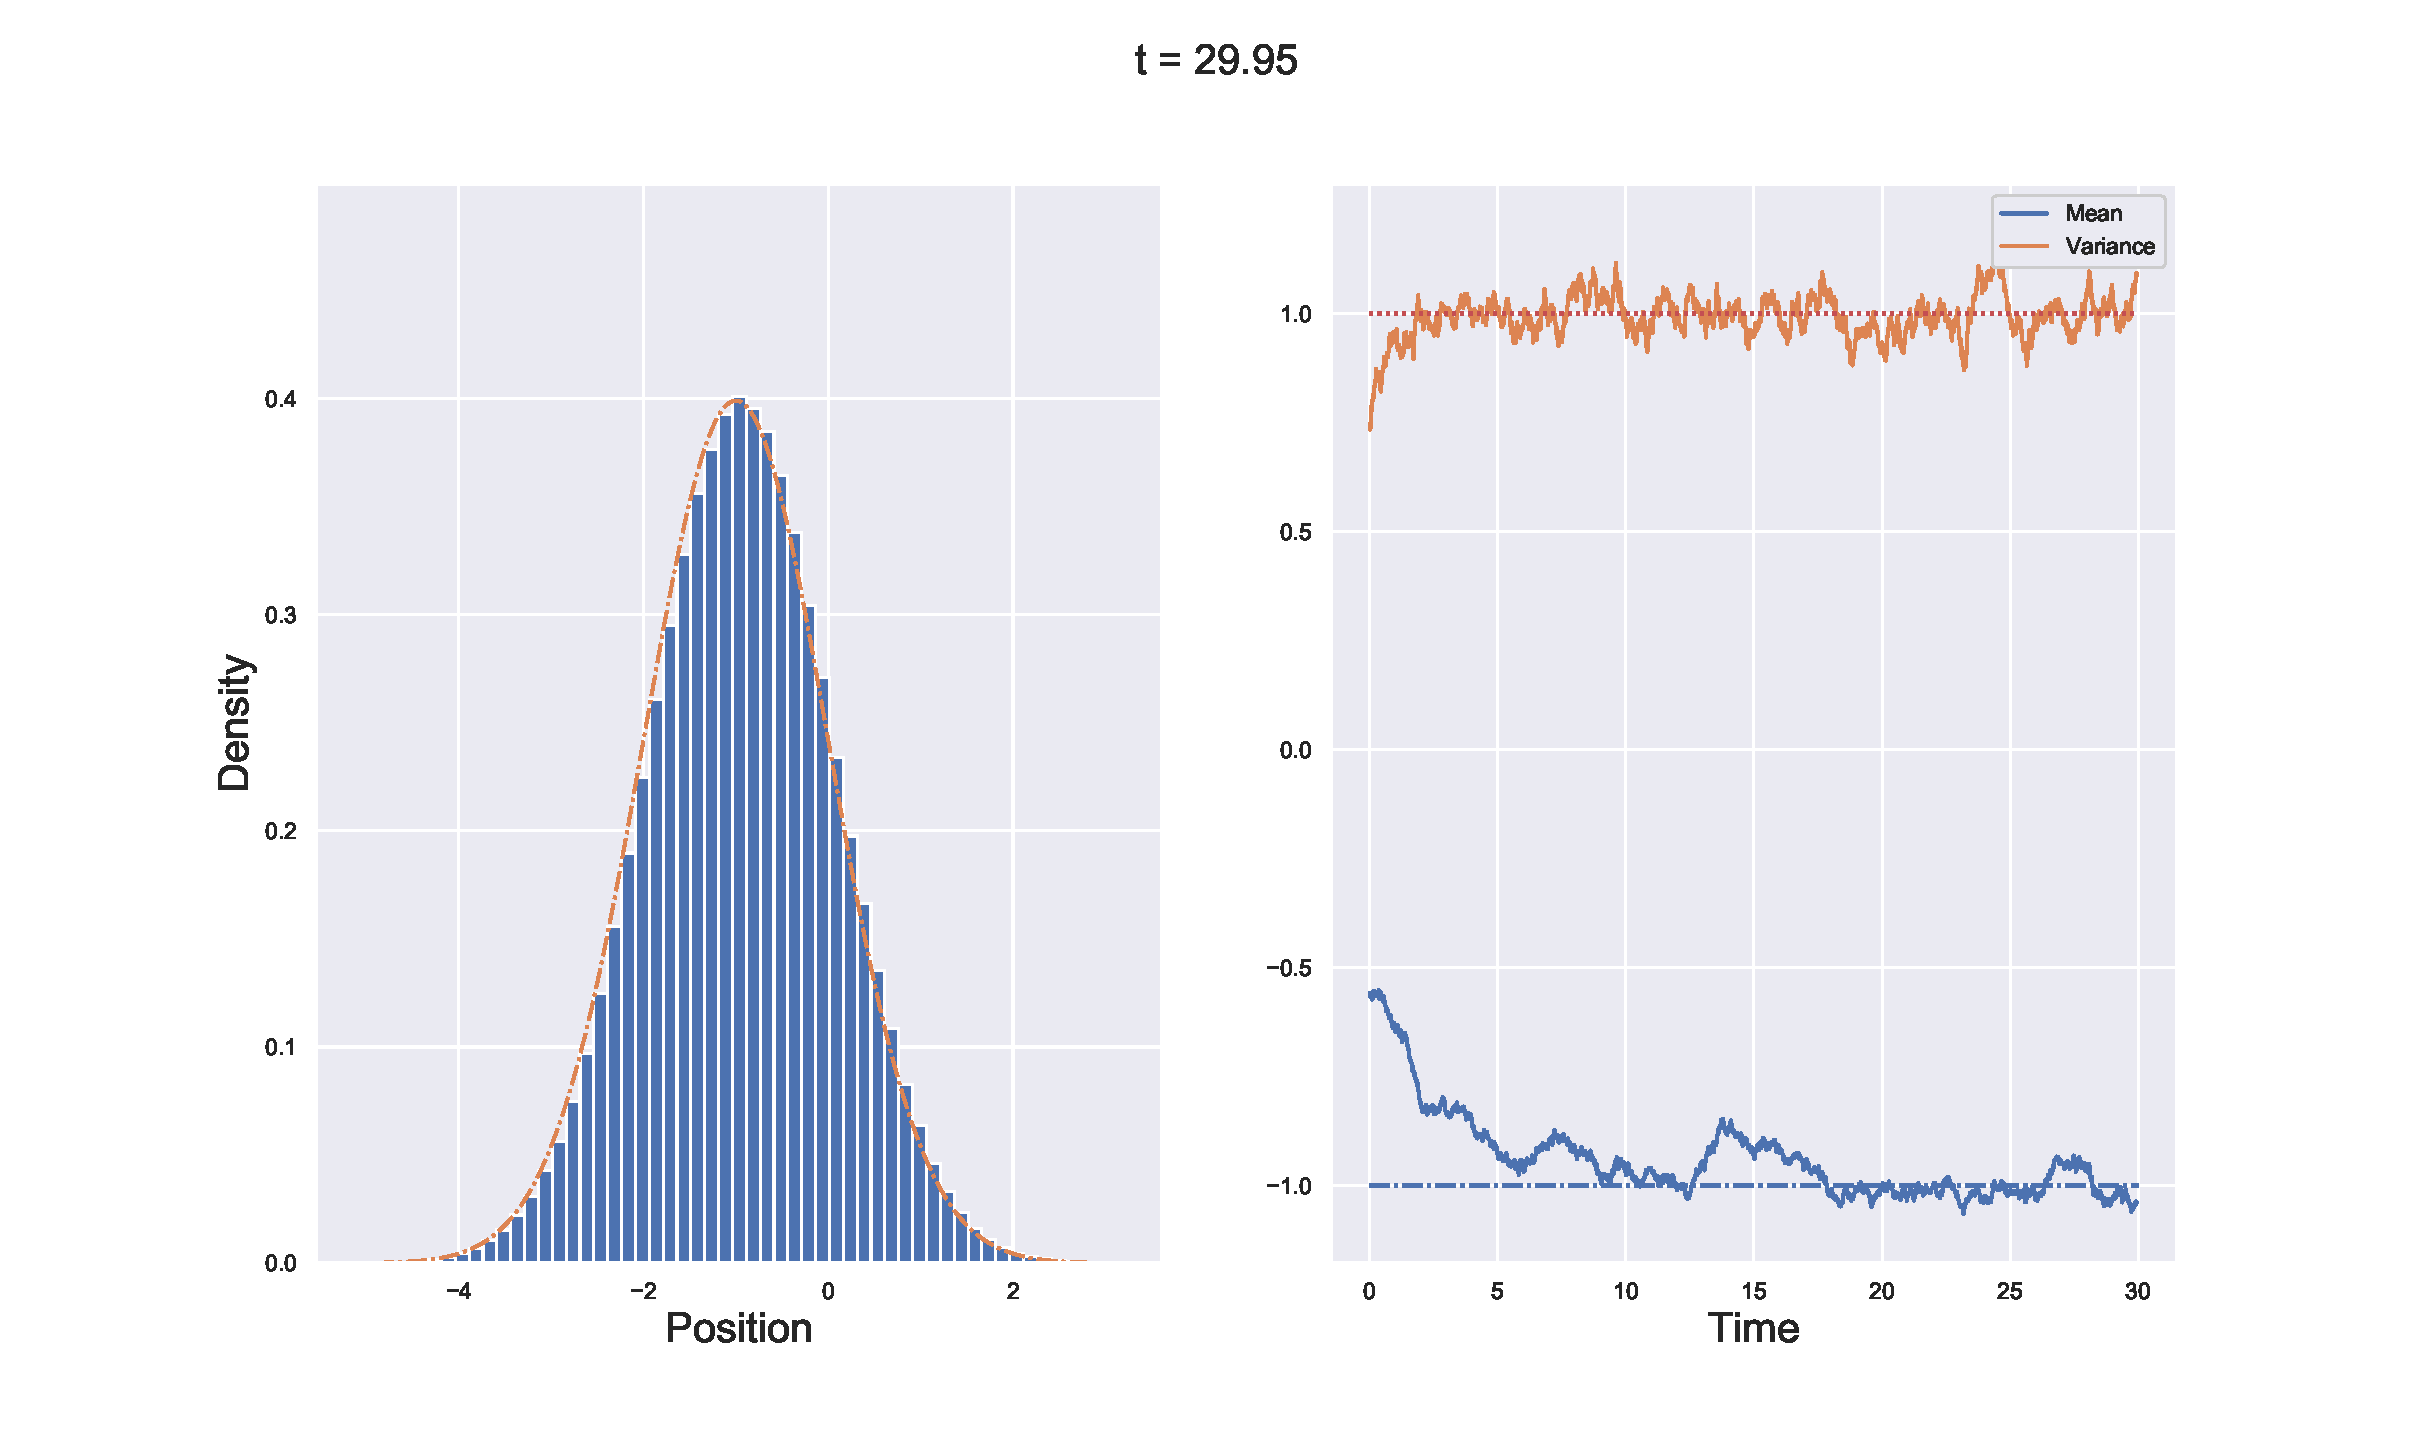
\includegraphics[width=\linewidth]{Figures/homparticles}
    \caption[Homogeneous Particle System]{Histogram of velocities of 1000 particles after 30s with $\sigma = 1$ against the analytic stationary distribution. A time step of $\Dt = 0.01$ was used and the initial data was uniform on $[-2,1]$. The right-hand plot shows the mean and variance moving towards the predicted values and oscillating about them.}
    \label{fig:homparticlemoments}
\end{figure}
We can also plot an animation of the movement of the density of particles over time. Recall from Section \ref{sec:dynamics} that the empirical distribution of the particle system only approximates the true distribution as the number of particles tends to infinity. For any finite number of particles there is only one stationary distribution. When simulating the system, if the number of particles is high enough the probability that enough particles jump across the barrier is very small, and will only be seen if the simulation is ran for an extremely long time. Nevertheless, if the number of particles is low enough, these switches happen often enough to observe, as Figure \ref{fig:switch} shows. This something to be aware of when comparing the kinetic model with the particle model -- a low number of particles produces a better approximation to the invariant distribution of the particle system, but a worse approximation of the kinetic model solution.

\begin{figure}
    \centering
    \includegraphics[width=\linewidth]{Figures/switch}
    \caption[Mean Zero Invariant Measure for the Particle System]{When simulated for a long time with a low number of particles (here there are 6, and $T=500$) the particles do not behave as the kinetic model predicts.}
    \label{fig:switch}
\end{figure}

+++List of things that can be done in code?+++

\subsection{Space-Homogeneous Kinetic Model}\label{sec:homkin}
 Consider the space-homogeneous evolution given by \eqref{eq:spacehomPDE}, that is
    \begin{equation}
    \partial_t f_t(v) = \partial_v vf_t(v) - \partial_v G(\langle w \rangle_{f_t})f_t(v) + \sigma \partial_{vv} f_t(v).\tag{\ref{eq:spacehomPDE}}
    \end{equation}
    Using the methods developed in Section \ref{sec:numericalmethods}, we are now able to approximate this system numerically. As when solving the heat equation, a zero boundary condition shall be enforced. This is valid as we know that the stationary distributions are Gaussian and centred at $-1,0,+1$. The boundary $L$ can then be chosen depending on the the diffusion so that almost no mass is contained beyond the boundary. For example if $\sigma = 1$, the mass contained beyond $L=5$ is of the order $10^{-5}$. 
    
    Simpson's rule will be used as a quick way to approximate the integral within the herding coefficient. To differentiate between the integral and its approximation, we write \(\langle w\rangle_{F^n}\). Below is the scheme when both the herding coefficient and the velocity are positive, using a finite difference scheme with a CN discretisation for the diffusive term and an upwind method for the damping and herding terms.
    \begin{equation*}
    \begin{split}
    \frac{F_j^{n+1} - F_j^n}{\Delta t} = 	-G(\langle w\rangle_{F^n})\left[ \frac{F^n_{j+1} - F^n_{j}}{\Delta v}\right] &+\left[ \frac{v_{j}F^n_{j} - v_{j-1}F^n_{j-1}}{\Delta v}\right]\\ &+ \frac{\sigma}{2}\left[ \frac{F^{n+1}_{j+1} - 2F^{n+1}_j + F^{n+1}_{j-1}}{(\Delta v)^2} + \frac{F^{n}_{j+1} - 2F^{n}_j + F^{n}_{j-1}}{(\Delta v)^2}\right] 	 
    \end{split}
    \end{equation*}
    This scheme will be first order in both time and space due to the use of the first-order upwinding. The stability will be restricted by the CFL condition, in particular, $\frac{|v_j-G(\langle w\rangle_{F^n})|\Dt}{\Dx} \leq 1$. A finite volume scheme has also been implemented. In this scheme the flux out of the right boundary is given by 
     \[ \max(0, v_{j+\frac{1}{2}}-G(\langle w\rangle_{F^n}))F^n_{j+1} + \min(0, v_{j+\frac{1}{2}}-G(\langle w\rangle_{F^n}))F^n_j + \frac{\sigma(F^n_{j+1} - F^n_j)}{\Dv}.
     \]
     This is a simple FTCS method applied to the diffusion term and a first order upwind on the advective term. The stability here is limited by the mesh spacing, however it illustrates the use of a finite volume method without incorporating an implicit solver. Figure +++ref+++ is a frame from an animation of the PDE solution approximated using the finite difference scheme compared with the particle system. The finite difference method appears to closely follow the behaviour of the particle system, so long as the number of particles is high enough. Figure \ref{fig:kinmodelmomvar} shows the first moment and the variance contrasted with the analytic solution of \eqref{eq:momode}. This clearly shows the almost immediate artificial dissipative effects of the upwind scheme in the finite volume case. The finite difference scheme appears to be better approximating the variance, however the spatial bias within this algorithm is not correct. Both schemes report no mass loss to 6 decimal places. This will be the case as long as the initial distribution does not have non-negligible mass at the boundary.
     
     The error in the approximate stationary distribution can be approximated by simply finding the difference between the analytic invariant measure and the approximate solution. Figure \ref{fig:homkinerror} shows exactly this for $\sigma = 1, \Dt = 0.001, T = 20, L=6, \Dv = 0.1$ and Gaussian initial data. The spatial bias in the finite difference method has introduced a bias in the error. No such bias exists for the upwinding in the finite volume solution, although the error is greater. This is very important for our aim in this project. If the initial data has mean zero, the scheme may always converge in the direction of the spatial bias, obscuring the true behaviour. 
    
    \begin{figure}
        \centering
        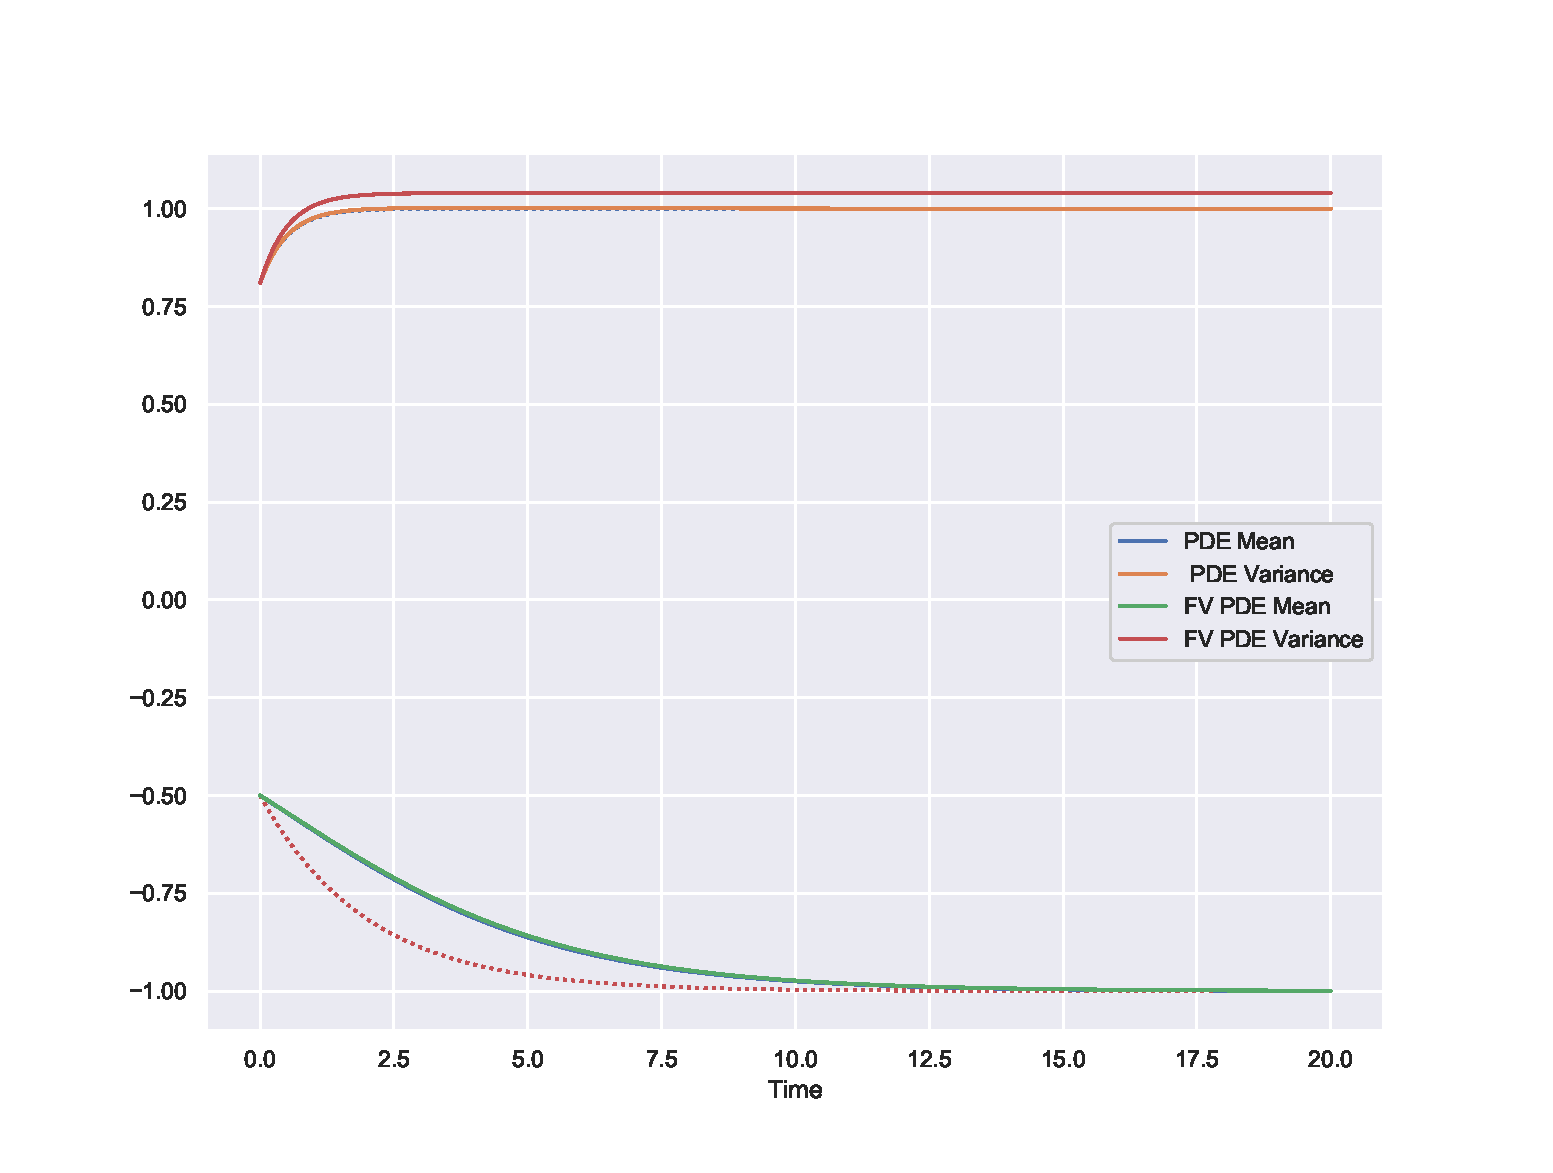
\includegraphics[width=0.7\linewidth]{Figures/kinmodelmomvar}
        \caption[Convergence of Moments for Kinetic Model]{For Gaussian initial data with mean -0.5 and variance 0.81, the schemes both converge with a time step of $\Dt =0.001$ and $\Dv = 0.05$. For the mean, the solvers are almost indistinguishable. The time step must be small so the FTCS scheme within the finite volume solver is stable. Also note the overestimation of variance. }
        \label{fig:kinmodelmomvar}
    \end{figure}

    \begin{figure}
        \centering
        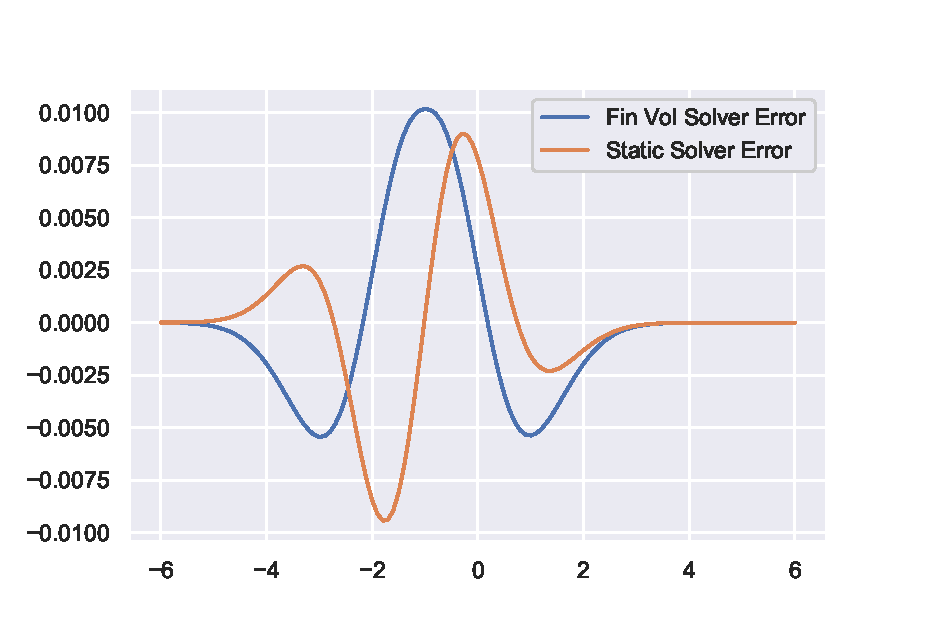
\includegraphics[width=0.7\linewidth]{Figures/homkinerror}
        \caption[Error of the Schemes]{Difference between approximate solution at $t=20$ and a Gaussian distribution with mean -1 and variance 1. Note the spatial bias in the finite difference method has introduced a bias in the error. No such bias exists for the upwinding in the finite volume case.}
        \label{fig:homkinerror}
    \end{figure}
\subsection{Space-Heterogeneous Particle Model}\label{sec:hetkin}
    The next step is to reintroduce the spatial heterogeneity in the particle system. Recall the full particle model is given by
            \begin{equation}\begin{cases}
    \dif x^{i,N}_t = v^{i,N}_t\dif t\\
    \dif v^{i,N}_t = -v^{i,N}_t\dif t + G\left(\frac{\frac{1}{N}\sum_{j=1}^N \phi(x_t^{i,N} - x_t^{j,N})v^{j,N}_t  }{\frac{1}{N}\sum_{j=1}^N \phi(x_t^{i,N} - x_t^{j,N})}\right)\dif t + \sqrt{2\sigma} \dif W^i_t 
    \end{cases}, \qquad  i = 1,\dots,N.\tag{\ref{eq:fullparticle}}
    \end{equation} 
    Letting $\phi\equiv 1$ forces the interaction to be homogeneous in space still, however there is now the movement of particles in space given by the first equation. 
    
        
    \section{Discussion + Conclusion}\label{sec:conclusion}
            +++ future add other phi, recalc M +++

    \bibliographystyle{abbrv}
    \bibliography{whales.bib}
    \appendix
    \section{Thomas Algorithm}

\end{document}